\documentclass[a4paper,twocolumn,dvipdfm]{article}

% Učitaj pakete za kodnu stranicu utf8 i hrvatski jezik.
\RequirePackage[utf8]{inputenc}
\RequirePackage[croatian]{babel}

% Paket za hrvatski jezik neispravno izostavlja točke iza naslova,
% to ispravljamo zadavanjem novih funkcija za numeriranje koje stavljaju
% točku.
\makeatletter
\renewcommand\thesection{\@arabic\c@section.}
\renewcommand\thesubsection{\thesection\@arabic\c@subsection.}
\renewcommand\thesubsubsection{\thesubsection\@arabic\c@subsubsection.}
\renewcommand\theequation{\@arabic\c@equation}
%\renewcommand\thefigure{\@arabic\c@figure.}
%\renewcommand\thetable{\@arabic\c@table.}
\makeatother

% Ostali korisni paketi.
\RequirePackage{graphicx}
\RequirePackage[unicode]{hyperref}
\RequirePackage{amssymb}
\RequirePackage{amsmath}
\RequirePackage{pstricks}
\RequirePackage{booktabs}
\RequirePackage{multirow}




% Ovdje započinje članak.
\begin{document}

% Navedite naslov i autore. Datume se automatski postavlja na datum kreiranja dokumenta,
% no može se promijeniti zadavanjem \date{30. veljače, 2004.}
\title{Raspoznavanje rukom pisanih slova na ispitnim obrascima} 
\author{Tomislav Grbin, Mihej Komar, Ivan Kravarščan, Toni Pivčević i Ivana Stokić}
\maketitle

% Svako poglavlje započinje sa \section{Ime poglavlja} ako želimo da bude
% numerirano, a sa \section*{Ime poglavlja} ako ne želimo da bude numerirano.

\section*{Sažetak}
Sažetak od stotinjak riječi spominje najvažnije teme koje su obrađene u daljnjem
tekstu. TODO

\section{Uvod}
Klasifikacija
Uvod sadrži kratki opis područja, zašto je ono važno i koje su primjene. TODO

\section{Opis područja i aktivnosti u svijetu}
Opis područja je dataljniji prikaz područja uljučujući teoretske osnove i
primjene. TODO \cite{vamvakasoptical}

\begin{figure*}
\centering
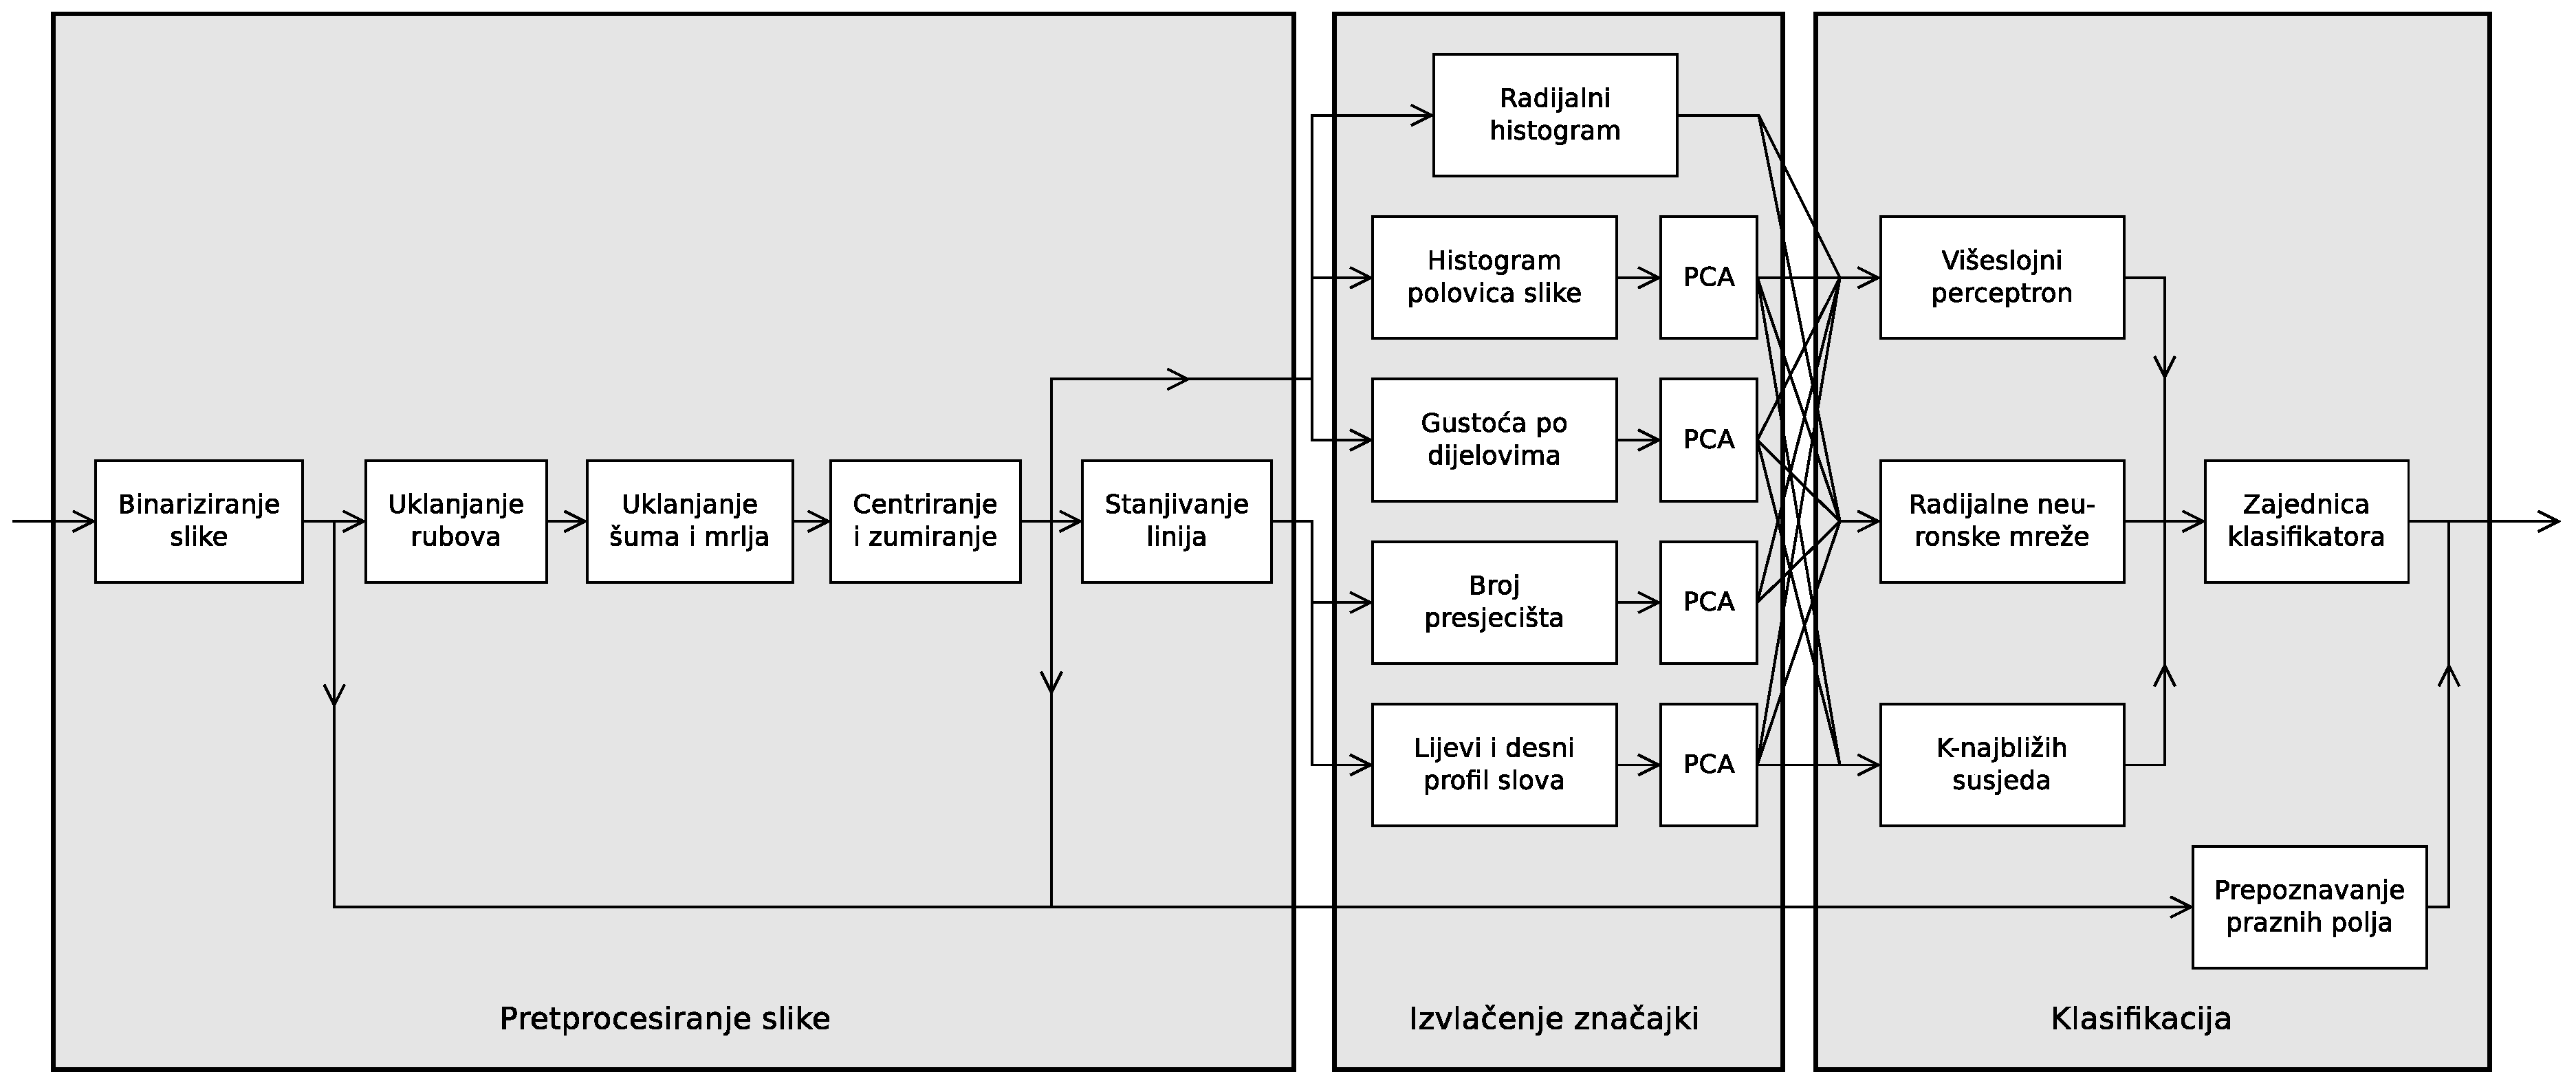
\includegraphics[width=\textwidth]{Diagram1.eps}
\caption{A caption}
\label{figure:alabel}
\end{figure*}

\section{Pretprocesiranje slike}
Prije izlučivanja značajki slova, potrebno je izvršiti pretprocesiranje slike.
Pretprocesiranje se sastoji od više koraka: binarizacije, uklanjanja rubova,
šuma i mrlja, centriranje i zumiranje slova te stanjivanja svih linija. S
obzirom na to da ispitni obrasci mogu biti skenirani različitim razlučivostima,
a slova mogu biti različitih veličina, debljina, intenziteta linija i pozicija u
polju, za precizno i kvalitetno izlučivanje značajki je potrebno svesti sva
slova na istu veličinu, debljinu i poziciju. Dobivene slike su identičnih
veličina (korištena je veličina 50x50), a slova su raširena preko cijele slike.

\subsection{Binariziranje slike}

\subsection{Uklanjanje rubova}

\subsection{Uklanjanje šuma i mrlja}
Uklanjanje šuma je izvedeno prema postupku koji su opisali K.\ Chinnasarn et.\
al.\ \cite{chinnasarn2002removing} čime se u jednom prolazu znatno smanjuju
manje skupine crnih piksela na bijeloj, bijelih piksela na crnoj podlozi i
rubovi slova se zaglađuju. Postupak je primijenjen s parametrom $k = 5$.
Primijećeno je da se u rijetkim slučajevima pojavljuju artefakti, ali nisu imali
veći utjecaj na rezultate klasifikacije. Problem su stvarala i slova A koja, ako
su napisana debelom linijom, u nekim slučajevima gube bijelu površinu u sredini
slova.

Ponekad i nakon uklanjanja šumova ostaju razne skupine piksela koje nisu dio
slova. Drugi dio ovog filtra uklanja upravo takve mrlje (točke, crtice i slične
oblike koje su udaljene od slova). Prvi korak algoritma je prepoznavanje
povezanih skupina piksela. Zatim se za najveću skupinu smatra da je glavni dio
slova. Nakon toga se gledaju udaljenosti između različitih skupina. Veće i
bliže skupine dijelovima slova smatraju se novim dijelom slova, a manje i dalje
skupine se smatraju mrljom i brišu se iz slike.

\subsection{Centriranje i zumiranje slova}

\subsection{Stanjivanje linija}


\section{Izlučivanje značajki}
Kako bi klasifikacija bila što preciznija, napravljeno je više različitih načina
izlučivanja značajki. Svaka metoda ima svoje prednosti i nedostatke, a
korištenjem različitih metoda rezultati klasifikacije mogu biti znatno bolji
nego korištenjem samo jedne metode klasifikacije.

Većina korištenih metoda izlučivanja značajki vraća vrijednosti iz
visokodimenzionalnog prostora s kojim bi klasifikacija bila manje kvalitete i
brzine. Zbog toga se koristi jedna od najčešćih metoda smanjivanja
dimenzionalnosti pomoću analize glavnih komponenti (engl.\ \emph{principal
component analysis}).

\subsection{Gustoća po dijelovima slike}
Izlučivanje značajki iz gustoće po dijelovima slike je najjednostavnija metoda
izlučivanja značajki. Slika se horizontalno i vertikalno dijeli na jednake
dijelove, a svaki dio se predstavlja odnos broja crnih i bijelih piksela realnim
brojem od 0 do 1. Broj 0 predstavlja da u tom dijelu nema crnih piksela, a 1
predstavlja da nema bijelih piksela. U klasifikaciji je podjela izvedena na 400
dijelova (20 horizontalnih i 20 vertikalnih), a dimenzionalnost se smanjuje
analizom glavnih komponenti na 20 dimenzija.

\subsection{Broj presjecišta}

\subsection{Histogram polovica slike}

\subsection{Radijalni histogram}

\subsection{Lijevi i desni profil slova}

\subsection{Hu-ovi invarijantni momenti}
TODO - napisati, ali uz napomenu da nisu bili zadovoljavajući rezultati


\section{Klasifikacija}

\subsection{Prepoznavanje praznih polja}

\subsection{Višeslojni perceptron}

\subsection{Radijalne neuronske mreže}

\subsection{Samoorganizirajuće mreže}
TODO - napisati da su isprobane i da nisu bile dobre

\subsection{K-najbližih susjeda}

\subsection{Zajednica klasifikatora}


\section{Rezultati}
U aplikaciji je korišteno 48 ispunjenih i jedan neispunjen ispitni obrazac koji
su skenirani rezolucijama 200 dpi i 300 dpi. Neka slova su namjerno napisana
izrazito neuredno i nečitko kako bi bilo moguće provjeriti kako se aplikacija
ponaša na takvim uzrocima. Potrebno je napomenuti kako se u praktičnim uvjetima
ne očekuje da će se na ulaz aplikacije davati izrazito nečitka slova. Ovim
postupkom je dobiveno ukupno 5864 slike slova koje su korištene za klasifikaciju
(skup S). Za skup za učenje (skup U) i testiranje (skup T) su korištene slike
skenirane višim rezolucijama bez slova koja su jako loše napisana. Također,
u ta dva skupa se ne koriste prazna polja jer se takva slova klasificiraju
posebnim klasifikatorom. Skup za učenje čini slučajno odabranih 80\% tog
podskupa slova, ali tako da udio svih slova ostane jednak. U Tablici
\ref{table:brojSlova} je prikazan broj slova po skupovima.

\begin{table}[htb]
\centering
\begin{tabular}{lrrr} \toprule
Slovo & T & U+T & S \\ \midrule
prazno & 0 & 0 & 144 \\
- & 78 & 391 & 796 \\
A & 60 & 303 & 622 \\
B & 51 & 256 & 532 \\
C & 49 & 247 & 505 \\
D & 46 & 230 & 467 \\
E & 46 & 234 & 492 \\
F & 46 & 234 & 488 \\
G & 44 & 222 & 462 \\
H & 43 & 215 & 460 \\
I & 42 & 212 & 437 \\
J & 44 & 221 & 459 \\ \midrule
Ukupno & 549 & 2.765 & 5.864 \\ \bottomrule
\end{tabular}
\caption{Broj slova po skupovima}
\label{table:brojSlova}
\end{table}

U aplikaciji je korišteno ukupno 13 klasifikatora koji čine različite
kombinacije izlučenih značajki slike i klasifikatora. U Tablici
\ref{table:rezPoKlasif} se mogu vidjeti rezultati prema svim korištenim
klasifikatorima. Uzorak je klasificiran na način da je odabran onaj razred s
najvećom vjerojatnošću. Najbolje rezultate pokazuju radijalne neuronske mreže, a
svi korišteni klasifikatori imaju točnost veću od oko 85\%. Ovi rezultati se
odnose na skup za testiranje. Zadnji red prikazuje rezultat za zajednicu
klasifikatora i može se primijetiti kako sinergija svih klasifikatora daje
znatno bolje rezultate od bilo kojeg pojedinačnog klasifikatora. Iz toga se može
zaključiti kako su različite metode izlučivanja značajki dovoljno nekorelirane
pa njihovim kombiniranjem se dolazi do znatno boljih rezultata.

\begin{table}[htb]
\centering
\begin{tabular}{llr} \toprule
Klasifikator & Značajke & Točnost \\
\midrule
\multirow{5}{2cm}{Višeslojni perceptron}
 & Presjecišta & 86,70\% \\
 & Gustoća & 88,34\% \\
 & Histogram & 84,88\% \\
 & Profili & 88,89\% \\
 & Radijalni hist. & 88,52\% \\
\midrule
\multirow{5}{2cm}{Radijalne neuronske mreže}
 & Presjecišta & 87,25\% \\
 & Gustoća & 93,99\% \\
 & Histogram & 92,90\% \\
 & Profili slova & 94,54\% \\
 & Radijalni hist. & 93,26\% \\
\midrule
\multirow{3}{2cm}{K-najbližih susjeda}
 & Histogram & 88,16\% \\
 & Gustoća & 90,89\% \\
 & Profili & 88,53\% \\
\midrule
\multirow{1}{2cm}{Zajednica}
 & Sve & 97,45\% \\
\bottomrule
\end{tabular}
\caption{Broj slova po skupovima}
\label{table:rezPoKlasif}
\end{table}

Rezultati za zajednicu klasifikatora po ostalim skupovima uzoraka se može
vidjeti u Tablici \ref{table:rezultati}. Očekivano je kako najveću točnost ima
skup koji uključuje uzorke za učenje i testiranje.

\begin{table}[htb]
\centering
\begin{tabular}{lrrr} \toprule
 & T & U+T & S \\ \midrule
Ispravno & 535 & 2.739 & 5.715 \\
Neispravno & 14 & 26 & 149 \\
Točnost & 97,45\% & 99,06\% & 97,46\% \\ \bottomrule
\end{tabular}
\caption{Klasifikacija bez korištenja nesigurnosti}
\label{table:rezultati}
\end{table}

S obzirom na to da je jedan od zahtjeva aplikacije što je moguća manja pogreška
čak pod cijenu ručnog klasificiranja dijela uzoraka, određena je metoda
kako se neki rezultat smatra sigurnim ili nesigurnim. Rezultat se smatra
sigurnim ako je vjerojatnost najvjerojatnijeg slova veća od 53\% ili omjer dva
najvjerojatnija slova veća od 1,75. Ako se na ovaj način izvede klasifikacija,
dodatno se podiže točnost klasifikacije na 99,41\%. Rezultati za sve korištene
skupove uzoraka prikazani su u Tablici \ref{table:rezultati2}.

\begin{table}[htb]
\centering
\begin{tabular}{lrrr} \toprule
 & T & U+T & S \\ \midrule
Ispravno & 508 & 2678 & 5.533 \\
Neispravno & 3 & 4 & 51 \\
Nesigurno & 38 & 83 & 280 \\
Udio nesigurnih & 6,92\% & 3,00\% & 4,77\% \\
Točnost sigurnih & 99,41\% & 99,85\% & 99,09\% \\ \bottomrule
\end{tabular}
\caption{Klasifikacija s korištenjem nesigurnosti}
\label{table:rezultati2}
\end{table}

Dodatno podizanje točnosti klasifikacije se može postići tako da se prilikom
klasifikacije definira koja slova se očekuju kao rezultat. Primjerice, ako neki
ispitni obrasci imaju definirane odgovore od A do F, što je jedna od najčešće
korištenog broja odgovora, tada nije potrebno određivati vjerojatnosti slova od
G do J. U aplikaciji je to izvedeno kao ograničavanje izlazne dimenzionalnosti.
Prva dimenzija određuje vjerojatnost za prazno polje, druga za crticu, a od
treće do dvanaeste za slova od A do J. Na Slikama \ref{figure:rezPoDim1} i
\ref{figure:rezPoDim2} je prikazana točnost klasifikacije po broju dimenzija. Na
Slici \ref{figure:rezPoDim1} je klasifikacija bez korištenja nesigurnosti, a na
Slici \ref{figure:rezPoDim2} s korištenjem nesigurnosti. Iz grafa se može
očitati da ako postoje odgovori od A do F, tada je dimenzionalnost 8, a točnost
klasifikacije uz korištenje nesigurnosti je 99,72\%.

\begin{figure}
\centering
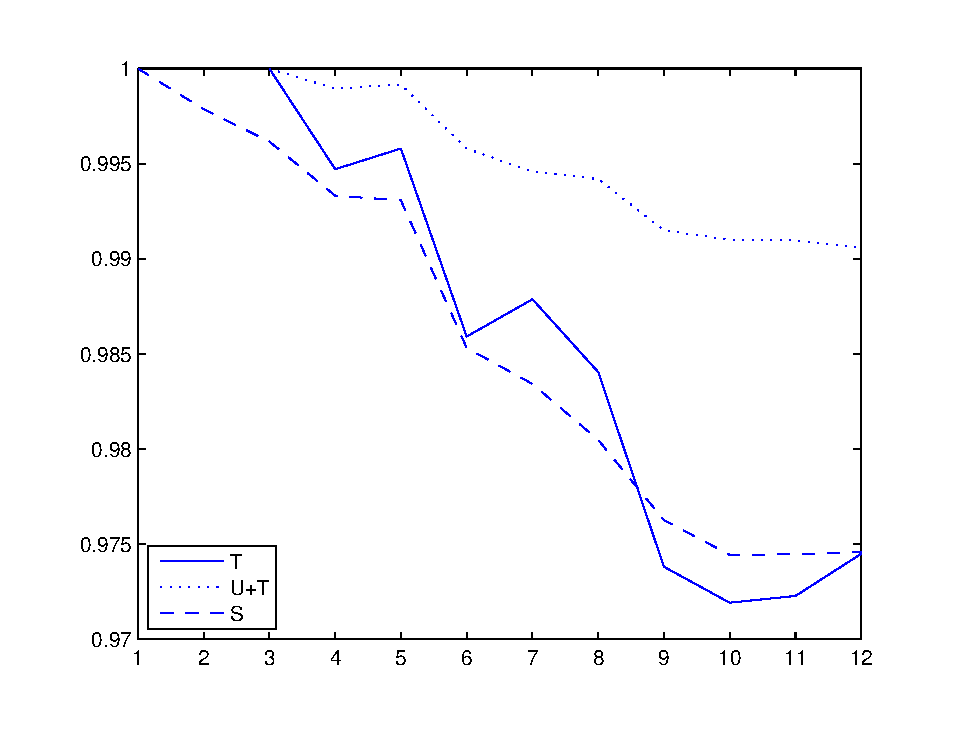
\includegraphics[scale=0.5]{accByDim1.eps}
\caption{Točnost klasifikacije po broju dimenzija bez upotrebe nesigurnosti}
\label{figure:rezPoDim1}
\end{figure}

\begin{figure}
\centering
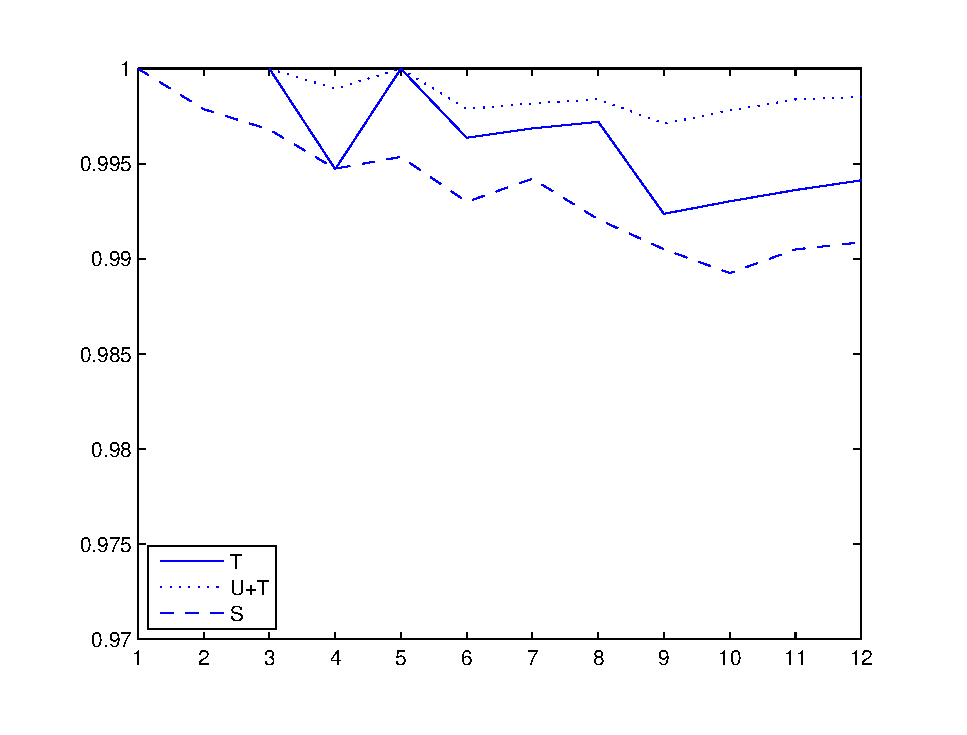
\includegraphics[scale=0.5]{accByDim2.eps}
\caption{Točnost klasifikacije po broju dimenzija uz upotrebu nesigurnost}
\label{figure:rezPoDim2}
\end{figure}

Na Slici \ref{figure:rezPoBrojuKlas} je prikazana točnost klasifikacije prema
broju korištenih klasifikatora. Iz grafa se može zaključiti kako dodavanjem
novih metoda izvlačenja značajki slike, klasifikatora i sličnog ne može znatno
povisiti udio ispravnih klasifikacija.

\begin{figure}
\centering
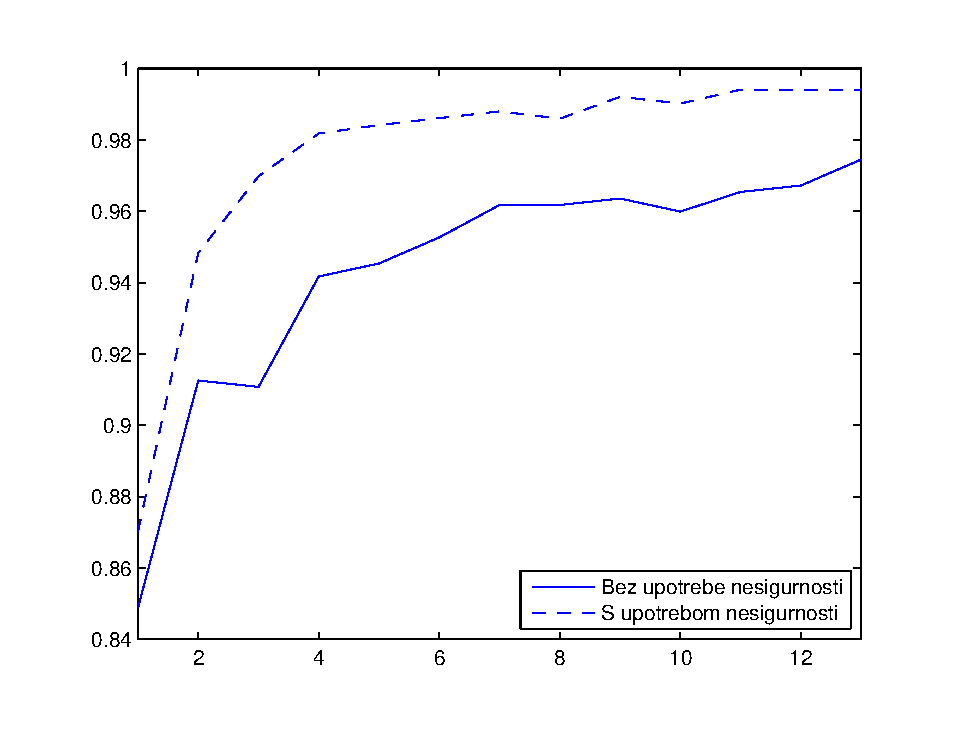
\includegraphics[scale=0.5]{accByClassifCount.eps}
\caption{Točnost klasifikacije po broju klasifikatora}
\label{figure:rezPoBrojuKlas}
\end{figure}


\section{Zaključak}
Zaključak treba istaknuti i diskutirati najvažnije rezultate iznesene u tekstu
i sugerirati eventualne buduće trendove. TODO

% Bibliografija
\bibliographystyle{amsplain}
\bibliography{literatura}

\end{document}